\section{簡介}
傳統的語意檢索是為了檢索純文字的文件,一個很成功的解決方式是查詢詞擴展 (Query Expansion)~\cite{tao2006regularized, lavrenko2001relevance, lv2009comparative}。當系統試圖對語音文件實作查詢詞擴展時,通常的實作方法是先將語音文件辨識成文字,再對這些文字文件套用查詢詞擴展,然而這種做法的缺點是辨識過程中不可避免地會出現辨識錯誤、辭典外詞彙而導致辨識結果不準確,進而影響到檢索結果。而且許多語音文件本身帶有的語音資訊如音高、聲調等等在被辨識成文字後就消失了且再也找不回來, 過去已有許多文獻使用聲學中的資訊以幫助語音文件檢索~\cite{parada2009query, norouzian2012exploiting, lee2012open, lee2011improved, lee2012integrating},而這也是本章想探討的方向。本章中提出的解決方法使用一套自動尋找的聲學組型 (Automatically Discovered Acoustic Patterns)~\cite{lee2012nonparametric, jansen2011towards, jansen2010towards, park2008unsupervised, stouten2008discovering, wang2011iterative, vanhainen2012word, driesen2012fast, zhang2010towards} 並將語音文件辨識成這些聲學組型的序列,而這些聲學組型是直接根據輸入信號的特性去尋找的,所以可以彌補文字查詢詞擴展在語音辨識階段損失的資訊,在過去已有文獻將聲學組型應用於語音文件分類 (Spoken Document Classification)~\cite{siu2010improved, hazen2011topic, gish2009unsupervised, chaudhuri2011unsupervised}、口述語彙偵測~\cite{lee2012nonparametric, huijbregts2011unsupervised, chan2011unsupervised, wang2012acoustic}、音樂檢索~\cite{riley2008text}和影片檢索~\cite{liu2010coherent}。

查詢詞擴展是一套基於虛擬回饋的架構,當使用者輸入文字形式的查詢詞後,系統會產生第一次檢索結果,並假設前 $N$ 篇都是與查詢詞虛擬相關 (Pseudo Relevant) 的,稱為虛擬相關文件 (Pseudo Relevant Document) 再根據最大概似估計 (Maximum Likelihood Estimation) 計算出最有可能與查詢詞語意相關的詞彙加入到查詢詞中。本章中將在這個架構上加上聲學組型的資訊用以解決以上所說的語音數位內容檢索會因為辨識錯誤、辭典外詞彙而導致檢索性能下降等問題。我們在此提出的架構將把語音文件同時辨識成文字的詞圖與聲學組型的唯一最佳序列,並同時於其上進行查詢詞擴展。根據文字上的第一次檢索結果可以得知哪些語音文件與查詢詞是虛擬相關,並假設那些常出現在虛擬相關文件中的聲學組型為與查詢詞語意相關的,再用這些聲學組型去檢索所有的聲學組型序列得到另一份檢索結果,最後由於聲學組型成效不如文字穩定,因此將此檢索結果與文字檢索結果疊加後可得穩定進步的成效。如此一來,即使文件中包含了辭典外詞彙或是辨識錯誤,也有可能可以從聲學組型的檢索中找出來。

\section{傳統監督式語音文件語意檢索}
\label{sec:chap4_semantic_retrieval}
語意檢索的目的是要找出所有與查詢詞語意上相關的文件,其中一種解決方式是查詢詞擴展 (Query Expansion) ,查詢詞擴展可以找出在目標文件集合中與查詢詞語意上相關的詞彙,並將其加入到原查詢詞的集合中,成為新的一組查詢詞,稱為擴展後的查詢詞 (Expanded Query) ,系統會自動使用這組新的查詢詞進行一次新的檢索,這次檢索回傳的文件就會包含擴展後的查詢詞,因此這些文件就會是與原查詢詞語意上相關的文件。

查詢詞擴展使用虛擬回饋的框架,檢索系統在使用者輸入文字形式的查詢詞後,會先檢索出第一次檢索結果,再假設排序結果的前 $N$ 篇都是與查詢詞虛擬相關的文件,再利用查詢詞擴展找出這些虛擬相關文件中較常共同出現的詞彙,卻又不是常常出現在所有文件中的詞彙,並將這些詞彙加入原查詢詞中,成為新的一組查詢詞,稱為擴展後查詢詞 (Expanded Query) ,系統再利用擴展後查詢詞進行下一次檢索後將結果回傳給使用者,即為傳統監督式語音文件語意檢索的做法。

方法細節簡介如下:

\subsubsection{前處理}
\label{sec:preprocessing}
本章使用的檢索方式主要是基於語言模型的檢索 (Language Modelling Retrieval),因此首先要把辨識所得的詞圖轉換為語言模型。對語音文件$x$中的每個詞$t$,它在詞圖中的期望出現次數 (Expected Count) 可以如此計算:

\begin{equation}
E[t|x] = \sum_{\mu \in L(x)} N(t, \mu)P(\mu|x)
\end{equation}

$L(x)$是$x$的詞圖中所有的路徑,$\mu$是$L(x)$中的一條路徑,$N(t, \mu)$是$t$在$\mu$中出現的次數,$P(\mu|x)$是路徑$\mu$的事後機率(Posterior Probability)。

有了$E[t|x]$之後,就能把詞圖表示成單連詞語言模型$\theta_x$:

\begin{equation}
P(t|\theta_x) = \frac{E[t|x]}{\sum_tE[t|x]}
\end{equation}

因為$\theta_x$裡沒有包含每個詞,為了讓$\theta_x$中每個詞都有一點機率,會再把$\theta_x$與一個背景語言模型 (Background Language Model) $\theta_b$做線性疊加,這個過程稱為平滑化,平滑化後的語音文件模型為$\bar{\theta}_x$。$\theta_b$可以如此估計:
\begin{equation}
\label{equ:chap3_bgm}
P(t|\theta_b) = \frac{\sum_{x\in C}E[t|x]}{\sum_t\sum_{x\in C}E[t|x]}
\end{equation}

其中 $C$ 是所有語音文件$x$的集合。

\subsection{第一次檢索結果}
\label{sec:chap3_fpr}
在此,我們將使用者輸入的文字查詢詞表示成語言模型$\theta_q$:
\begin{equation}
P(t|\theta_q) = \frac{N(t, q)}{|q|}
\end{equation}

$N(t, q)$ 是詞彙$t$在查詢詞$q$中出現的次數,$|q|$是查詢詞$q$中所有的詞彙總數。第一次檢索結果是由排序以下分數$S_0(q, x)$得到:

\begin{equation}
\label{equ:chap3_fpr}
S_0(q, x) = -[(1-w_1)KL(\theta_q^{w}|\bar{\theta}_x^{w}) + w_1KL(\theta_q^{s}|\bar{\theta}_x^{s})]
\end{equation}

上式同時使用了詞單位的語言模型$\theta_q^w, \bar{\theta}_x^{w}$和次詞 (Subword) 單位的語言模型$\theta_q^{s}, \bar{\theta}_x^{s}$。$w_1$是線性疊加兩者時的權重,通常我們使用 $w_1 = 0.95$。並取其中的前 $N$ 篇為虛擬相關文件,進行下一步的查詢詞擴展。

\subsection{查詢詞擴展與第二次檢索}
這裡使用的查詢詞擴展訓練方法同~\ref{sec:prf},經過查詢詞擴展後,即可得到擴展後查詢詞模型$\theta_{qe}$,在擴展後查詢詞模型中,會包含許多常一起出現在虛擬相關文件中,但不會常出現在所有文件中的詞,而這些詞通常會是與原查詢詞成語意相關的,因此再用這套擴展後查詢詞模型進行第二次檢索 (Second-pass Retrieval),即可檢索到更多與原查詢詞語意相關的文件,第二次檢索的相關分數 $S(q, x)$ 為:

\begin{equation}
S_0(q, x) = -[(1-w_1)KL(\theta_{qe}^{w}|\bar{\theta}_x^{w}) + w_1KL(\theta_{qe}^{s}|\bar{\theta}_x^{s})]
\end{equation}

這裡也是同時使用了詞單位的語言模型$\bar{\theta}_x^{w}$和次詞 (Subword) 單位的語言模型$\bar{\theta}_x^{s}$。$w_1$是線性疊加兩者時的權重,通常我們使用 $w_1 = 0.95$。

將所有語音文件 $x$ 按照其與查詢詞 $q$ 的相關分數 $S(q, x)$ 排序後即可得到第二次檢索結果 (Second-pass Retrieval Result),再將其呈現給使用者。

\section{以聲學組型改善監督式語意檢索}
上一節提到的傳統監督式語意檢索確實可以很好地找出與查詢詞語意上相關的文件,但由於語音文件被辨識成文字文件時很有可能會出現辨識錯誤,或某些詞彙可能是辭典外詞彙,進而使得查詢詞擴展遇到困難。事實上當系統將語音文件辨識成文字文件時,就已經損失了很多資訊,並且這些資訊是再也找不回來的了,因此這節的目的是要利用這些聲學的資訊彌補查詢詞擴展。

本論文提出了一個系統解決以上的問題,如圖 ~\ref{fig:chap3_system}。在圖 ~\ref{fig:chap3_system}的左下角系統會自動從所有文件的集合中學出一套類詞單位和類次詞單位 的聲學組型的聲學模型和語言模型,再將語音文件用這套聲學組型辨識出來。因此圖 ~\ref{fig:chap3_system} 中的下半部將每個語音文件都表示成兩種格式:由語音辨識系統辨識而成的詞圖(包含詞與次詞兩種單位的詞圖)、由聲學組型組成的聲學組型串列。

當使用者輸入一個文字的查詢詞時,系統會將查詢詞與詞圖作比對 (圖中的右邊偏下) 並產生第一次檢索結果,系統並不會將這套第一次檢索結果回傳給使用者,而是假設其中的前
$N$篇是與查詢詞虛擬相關的,系統再利用這些虛擬相關文件作查詢詞擴展並用新的查詢詞模型檢索出一套新的檢索結果。接下來用聲學組型再做一次查詢詞擴展,即可得到聲學組型的查詢詞模型,聲學組型的查詢詞擴展假設其虛擬相關文件與文字的查詢詞擴展時相同,於是可得另一份新的查詢詞模型並用其檢索出另一套新的檢索結果,最後再把兩份檢索結果做線性疊加再排序後回傳給使用者。如此一來,即使在文字的查詢詞擴展時有些詞彙被錯誤地辨識或是有辭典外詞彙,也可以透過聲學組型的查詢詞擴展將對應到這些詞的聲學組型加到聲學組型的查詢詞模型中,於是仍然可以找到包含有這些詞彙的文件。

\begin{figure}
\centering
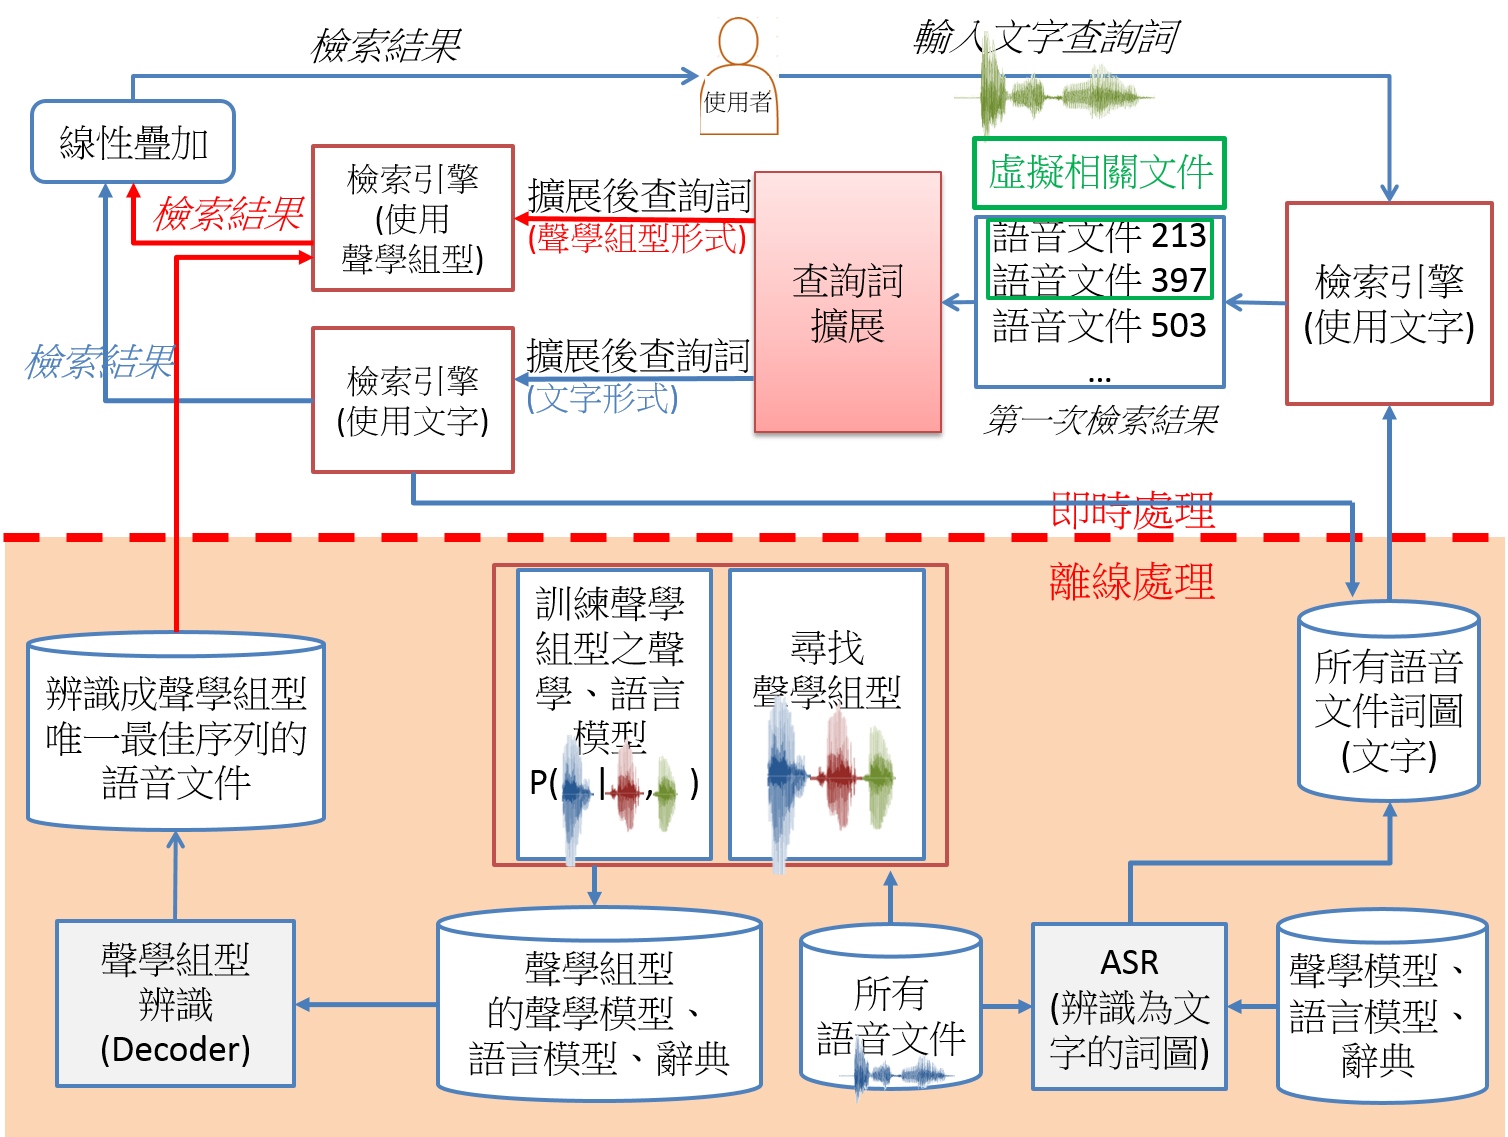
\includegraphics[scale=0.5]{images/chap3_system_zh.png}
\caption{系統架構示意圖} \label{fig:chap3_system}
\end{figure}

\subsection{前處理}
\subsubsection{文字語言模型}
此處文字形式的前處理方式同~\ref{sec:preprocessing}。因此要先把語音文件 $x$ 辨識為詞單位的詞圖與次詞單位的詞圖後,再將詞圖轉換為詞單位的語言模型 $\bar{\theta}_x^w$ 與次詞單位的語言模型 $\bar{\theta}_x^s$。以下舉詞單位的詞圖為例,對語音文件$x$中的每個詞$t$,它在詞圖中的期望出現次數 (Expected Count) 可以如此計算:

\begin{equation}
E[t|x] = \sum_{\mu \in L(x)} N(t, \mu)P(\mu|x)
\end{equation}

$L(x)$是$x$的詞圖中所有的路徑,$\mu$是$L(x)$中的一條路徑,$N(t, \mu)$是$t$在$\mu$中出現的次數,$P(\mu|x)$是路徑$\mu$的事後機率(Posterior Probability)。

有了$E[t|x]$之後,就能把詞圖表示成單連詞語言模型$\theta_x^w$:

\begin{equation}
P(t|\theta_x^w) = \frac{E[t|x]}{\sum_tE[t|x]}
\end{equation}

因為$\theta_x^w$裡沒有包含每個詞,為了讓$\theta_x^w$中每個詞都有一點機率,會再把$\theta_x^w$與一個背景語言模型 (Background Language Model) $\theta_b^w$做線性疊加,這個過程稱為平滑化,平滑化後的語音文件模型為$\bar{\theta}_x^w$。$\theta_b^w$可以如此估計:
\begin{equation}
P(t|\theta_b^w) = \frac{\sum_{x\in C}E[t|x]}{\sum_t\sum_{x\in C}E[t|x]}
\end{equation}

其中 $C$ 是所有語音文件$x$的集合。

以上的過程將同時對詞單位與次詞單位的詞圖計算,即可得詞單位的語言模型$\bar{\theta}_x^w$與次詞單位的語言模型 $\bar{\theta}_x^s$。

\subsubsection{聲學組型語言模型}
\label{sec:chap3_apd}
聲學組型指的是在某個特定語料中時常重複出現的聲音,比如像中文的音節、字等單位,這些聲學組型可以被用在口述文件分類、口述語彙偵測、語音文件檢索等。這裡使用的是本實驗室過去提出的雙層式聲學組型 (Two-Level Acoustic Pattern)~\cite{chung2013unsupervised} (細節列於 ~\ref{sec:chap2_ap}),其中包含了類詞的聲學組型 (類詞聲學組型是由數個類次詞聲學組型所組成)和類次詞的聲學組型、類詞聲學組型如何由類次詞聲學組型組合而成的辭典、類詞聲學組型的$N$連語言模型 (N-gram Language
Model)。每個類次詞聲學組型就是一個隱藏式馬可夫模型,所有的隱藏式馬可夫模型的參數、類次詞聲學組型的數目、類詞聲學組型的數目和類詞聲學組型的$N$連語言模型都是在非監督式的狀況下自動地從語料庫學習出來的。學習出聲學組型以後,這些聲學模型、語言模型和辭典可以用來建立一個辨識系統,並將這些語音文件辨識成聲學組型的序列,如此即可將語音文件$x$表示成聲學組型的語言模型$\phi_x$:

\begin{equation}
P(v|\phi_x) = \frac{C(v, x)}{\sum_v C(v, x)}
\end{equation}

$C(v, x)$ 為聲學組型$v$在語音文件$x$中出現的次數。$\phi_x$會再與聲學組型背景語言模型$\phi_b$做平滑化(即線性疊加),平滑化的語音文件模型為$\bar{\phi}_x$。$\phi_b$表示如下:

\begin{equation}
P(v|\phi_b) = \frac{\sum_{x\in C} C(v, x)}{\sum_v\sum_{x\in C} C(v, x)}
\end{equation}

其中 $C$ 是所有語音文件$x$的聲學組型序列,$v$是任一聲學組型,$C(v, x)$為聲學組型$v$在語音文件$x$的聲學組型序列中出現的次數。

\subsection{第一次檢索結果}
由於查詢詞$q$是文字形式的,因此第一次檢索結果只能用查詢詞模型$\theta_q$與文字的文件模型$\bar{\theta}_x^w$ 和 $\bar{\theta}_x^s$做比對,而不能使用聲學組型的文件模型$\bar{\phi}_x$
。所以計算第一次檢索結果的相關分數$S_0(q, x)$同式 ~\ref{equ:chap3_fpr}為:
\begin{equation}
S_0(q, x) = -[(1-w_1)KL(\theta_q^{w}|\bar{\theta}_x^{w}) + w_1KL(\theta_q^{s}|\bar{\theta}_x^{s})]
\end{equation}

並取其中的前 $N$ 篇為虛擬相關文件,進行下一步的查詢詞擴展。

\subsection{查詢詞擴展}
以下簡介文字型式的查詢詞擴展與聲學組型形式的查詢詞擴展如下:

\subsubsection{文字形式的查詢詞擴展}
此處的查詢詞擴展與 ~\ref{sec:prf} 中類似,計算方法與式~\ref{equ:chap2_prf_f1f2}相似,只要最大化下式:

\begin{equation}
\label{equ:prf_f1f2_text}
F(\theta_{qe}, \alpha_{d_1}, ..., \alpha_{d_M}) = F_1(\theta_{qe}, \alpha_{d_1}, ..., \alpha_{d_M}) F_2(\theta_{qe})^\lambda
\end{equation}

其中 $F_1(\theta_{qe}, \alpha_{d_1}, ..., \alpha_{d_M})$ 定義如下:

\begin{equation}
\label{equ:chap3_prf_f1_text}
F_1(\theta_{qe}, \alpha_{d_1}, ..., \alpha_{d_M}) = \Pi^M_{m=1} \Pi_w (\alpha_{d_m} P(w|\theta_{qe}) + (1 - \alpha_{d_m}) P(w|\theta_b))^{P(w|\theta_{d_m})}
\end{equation}

上式中,產生詞彙 $w$ 的機率為 $\alpha_{d_m} P(w|\theta_{qe}) + (1-\alpha_{d_m}) P(w|\theta_b)$ 。因此上式可視為由新的查詢詞模型產生這些虛擬相關文件的可能性 (Likelihood)。然而,如果只最大化式~\ref{equ:chap3_prf_f1_text},$\theta_{qe}$ 中主要會包含這些虛擬相關文件的主題,而不一定是查詢詞相關的詞彙,為了要解決這個問題,比較好的方法是用原本的查詢詞模型 $\theta_q$ 正規化 (Regularize) $\theta_{qe}$,因此定義 $F_2(\theta_{qe})$ 如下:

\begin{equation}
\label{equ:chap3_prf_f2_text}
F_2(\theta_{qe}) = \Pi_w P(w|\theta_{qe})^{P(w|\theta_q)}
\end{equation}

當 $\theta_{qe}$ 和 $\theta_q$ 越近時,$F_2(\theta_{qe})$ 就會越大,因此如果我們同時最大化兩者的乘積即式~\ref{equ:prf_f1f2_text},就能夠同時將虛擬相關文件中的詞彙加進擴展後查詢詞,也能同時正規化這個過程,使得擴展後查詢詞不致於與原查詢詞相差太遠。正規化的強度由~\ref{equ:prf_f1f2_text}中的$\lambda$決定,$\lambda$越大,擴展後查詢詞 $\theta_{qe}$ 與 $\theta_q$ 就會被強制靠得越近,$\lambda$越小則反之。

$\theta_{qe}$ 即為擴展後的文字查詢詞模型,最大化~\ref{equ:prf_f1f2_text}的方法採用 EM 演算法:

E step: 對於${d_1, d_2, ..., d_M}$ 中的每篇語音文件$d_m$中的每一個詞彙 $w$:

\begin{equation}
\label{equ:prf_estep}
P(R|w, d_m) = \frac{\alpha_{d_m} P(w|\theta_{qe})}{\alpha_{d_m} P(w|\theta_{qe}) + (1-\alpha_{d_m}) P(w|\theta_b)}
\end{equation}

其中 $P(R|w, d_m)$ 為當給定文件 $d_m$ 中的詞彙 $w$ 時,此文件 $d_m$ 中的詞彙 $w$ 與查詢詞是語意上相關的機率。 

M step: 對於 ${d_1, d_2, ..., d_M}$ 中的每篇語音文件 $d_m$,其中每篇語音文件 $d_m$ 的語言模型為 $\theta_d$:

\begin{equation}
\label{equ:prf_mstep}
\alpha_{d_m} = \sum_w P(R|w, d_m)P(w|\theta_d)
\end{equation}

對每個詞彙 $w$:

\begin{equation}
P(w|\theta_{qe}) = \frac{\lambda P(w|\theta_q)+\sum^M_{m=1} P(w|\theta_d) P(R|w, d_m)}{\lambda + \sum_w \sum^M_{m=1} P(w|\theta_d) P(R|w, d_m)}
\end{equation}

重覆地執行 E Step 和 M Step 即可得到新的查詢詞模型 $\theta_{qe}$,以上的步驟必須同時對詞版本的詞圖與次詞版本的詞圖各進行一次,故會得到兩種版本的擴展後查詢詞,分別為詞版本的擴展後查詢詞 $\theta_{qe}^{w}$ 與次詞版本的擴展後查詢詞 $\theta_{qe}^{s}$。

\subsubsection{聲學組型形式的查詢詞擴展}
此處的查詢詞擴展也與 ~\ref{sec:prf} 中相似,但由於我們沒有聲學組型形式的原查詢詞,故此時不需要如上一小節乘上$F_2(\phi_{qe})$,所以是最大化下式:

\begin{equation}
\label{equ:prf_f1f2_acoustic}
F(\phi_{qe}, \alpha_{d_1}^{'}, ..., \alpha_{d_M}^{'}) = F_1(\phi_{qe}, \alpha_{d_1}^{'}, ..., \alpha_{d_M}^{'})
\end{equation}
由於聲學組型形式的$\alpha$與文字形式的$\alpha$不同,故以$\alpha^{'}$表示聲學形式的$\alpha$。其中 $F_1(\phi_{qe}, \alpha_{d_1}^{'}, ..., \alpha_{d_M}^{'})$ 定義如下:

\begin{equation}
\label{equ:chap3_prf_f1_acoustic}
F_1(\phi_{qe}, \alpha_{d_1}^{'}, ..., \alpha_{d_M}^{'}) = \Pi^M_{m=1} \Pi_v (\alpha_{d_m}^{'} P(v|\phi_{qe}) + (1 - \alpha_{d_m}^{'}) P(v|\phi_b))^{P(v|\phi_{d_m})}
\end{equation}

上式中,產生聲學組型 $v$ 的機率為 $\alpha_{d_m}^{'} P(v|\phi_{qe}) + (1-\alpha_{d_m}^{'}) P(v|\phi_b)$ 。因此上式可視為由新的查詢詞模型產生這些虛擬相關文件的可能性 (Likelihood)。

$\phi_{qe}$ 即為擴展後的文字查詢詞模型,最大化~\ref{equ:prf_f1f2_acoustic}的方法採用 EM 演算法:

E step: 對於${d_1, d_2, ..., d_M}$ 中的每篇語音文件$d_m$中的每一個聲學組型 $v$:

\begin{equation}
\label{equ:prf_estep}
P(R|v, d_m) = \frac{\alpha_{d_m}^{'} P(v|\phi_{qe})}{\alpha_{d_m}^{'} P(v|\phi_{qe}) + (1-\alpha_{d_m}^{'}) P(v|\phi_b)}
\end{equation}
其中 $P(R|v, d_m)$ 為當給定文件 $d_m$ 中的聲學組型 $v$ 時,此文件 $d_m$ 中的聲學組型 $v$ 與查詢詞是語意上相關的機率。 

M step: 對於 ${d_1, d_2, ..., d_M}$ 中的每篇語音文件 $d_m$,其中每篇語音文件 $d_m$ 的聲學組型語言模型為 $\phi_d$:

\begin{equation}
\label{equ:prf_mstep}
\alpha_{d_m}^{'} = \sum_v P(R|v, d_m)P(v|\phi_d)
\end{equation}

對每個聲學組型 $v$:

\begin{equation}
P(v|\phi_{qe}) = \frac{\sum^M_{m=1} P(v|\phi_d) P(R|v, d_m)}{\sum_v \sum^M_{m=1} P(v|\phi_d) P(R|v, d_m)}
\end{equation}

重覆地執行 E Step 和 M Step 即可得到聲學組型形式的擴展後查詢詞模型 $\phi_{qe}$

\subsubsection{線性疊加與第二次檢索}
有了文字的擴展後查詢詞模型$\theta_{qe}$與聲學組型的擴展後查詢詞模型$\phi_{qe}$後,由於聲學組型形式的擴展後查詢詞模型不如文字形式的擴展後查詢詞模型穩定,故需要線性疊加文字形式的第二次檢索與聲學組型形式的第二次檢索,因此整體的相關分數 $S(q, x)$ 計算如下:

\begin{equation}
\label{equ:prf_interpolation}
S(q, x) = -{(1-w_2)[(1-w_1)KL(\theta_{qe}^{w}|\bar{\theta}_x^{w}) + w_1KL(\theta_{qe}^{s}|\bar{\theta}_x^{s})] + w_2KL(\phi_{qe}|\bar{\phi}_x)}
\end{equation}

其中$w_2$為線性疊加時聲學組型形式的第二次檢索結果所佔的比重,$w_1$為使用詞版本的詞圖與次詞版本的詞圖時的比例,通常$w_1$使用$0.95$。

\section{實驗設定}
\label{sec:chap3_exp_design} 
本章的實驗使用的語料為2001年間從電台廣播中錄下的4小時新聞,並手動切成5034篇語音文件,每篇語音文件大約包含了$1至3$句的語句。用來辨識的語言模型是用1999年間收集的新聞文章 (包含4000萬個詞彙) 訓練而成,辭典中包含了62000個詞彙,聲學模型是用2000年間收集的8小時廣播新聞訓練而成的音節內(Intra-syllable) 右方資訊相依(Right-context-dependent) 聲韻母模型 (Initial-Final models)。辨識後的唯一最佳序列的字元正確率為 (Character Accuracy) 為75.27\%。
總共測試了29組查詢詞,每組查詢詞都有人工標注對應的語意相關文件,而這些語意相關文件中「並不一定要」包含查詢詞。本章中使用平均準確率做為評量標準。

\section{實驗結果及分析}

圖 ~\ref{fig:chap3_resulta} 中顯示的是式 ~\ref{equ:prf_interpolation} 疊加的結果,其中 $\lambda$ 固定為 800,$N$ 為 $5, 10, 15, 20, 25$ ,紅線則是第一次檢索結果,是不使用查詢詞擴展時的結果。縱軸是平均準確率(MAP),橫軸則是式 ~\ref{equ:prf_interpolation} 的$w_2$,為聲學組型與文字的擴展後查詢詞疊加時的權重,$w_1$在實驗中都被固定為 $0.95$。首先來比較第一次檢索結果與文字的查詢詞擴展後的結果 $(w_2 =
0)$時的狀況,可以觀察到文字的查詢詞擴展比第一次檢索結果好上一些,即使它可能有受到辨識錯誤或辭典外詞彙的影響。接下來看有使用聲學組型時的狀況:當 $w_2$大於零時,可以注意到整體的平均準確率相對 $w_2 = 0$時都是進步的 (只要$w_2 < 0.5$),這代表了使用聲學組型確實能夠幫助查詢詞擴展找到更多聲學方面的資訊,進而使平均準確率更為進步。另一方面也可以看到,當 N 增加,平均準確率會先成長後再下降,大約在 $N=10$
的時候為最佳的狀況,這個原因是由於當$N$變多時,被假設為虛擬相關的文件數也變多,因此更多的資訊被用來進行虛擬回饋,但另一方面如果假設了太多的虛擬文件時,會使用太多不相關資訊進行虛擬回饋,使得系統的平均準確率下降,最好的平均準確率是在 $N=10$而且 $w_2 = 0.40$ 的狀況,而這代表說文字的查詢詞擴展是比聲學組型的查詢詞擴展來得可靠的,因此文字查詢詞擴展的權重必須要設得高一些,由於這是最好的結果,所以在之後的實驗中會將 $N$ 設為 10。

圖 ~\ref{fig:chap3_resultb} 和圖 ~\ref{fig:chap3_resulta} 類似,只是圖 ~\ref{fig:chap3_resultb} 中將 $N$ 固定為 10,並且測試不同的 $\lambda$,在圖中可以發現當 $\lambda$ 很低的時候 (如100),系統的平均準確率甚至是比第一次檢索結果還要差的,然而當 $\lambda$ 夠大的話 ($\lambda \geq 400$),系統的平均準確率都是比第一次檢索結果和 $w_2 = 0$ 的狀況還要好的。這證明了式 ~\ref{equ:chap3_prf_f2_text} 的重要性,如果 $\lambda$ 太小的話就會導致系統在訓練時對於虛擬文件過適而使得成果更差,而 $\lambda$ 夠大時 ($\lambda > 400$) 就幾乎都能看到不錯的進步 。  

\begin{figure}
\centering
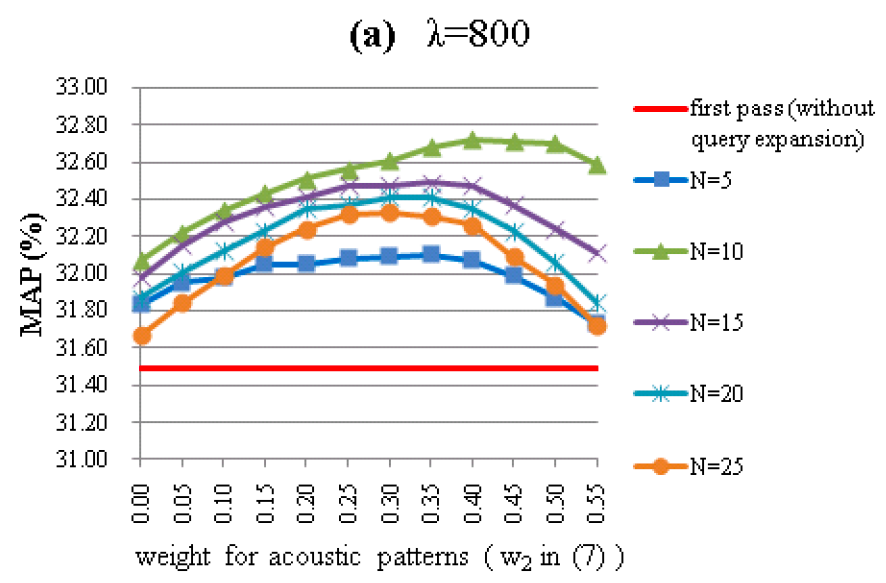
\includegraphics[scale=0.4]{images/chap3_resulta.png}
\caption{將文字形式和聲學組型形式的查詢詞擴展疊加後的平均準確率 ($\lambda = 800$)} \label{fig:chap3_resulta}
\end{figure}

\begin{figure}
\centering
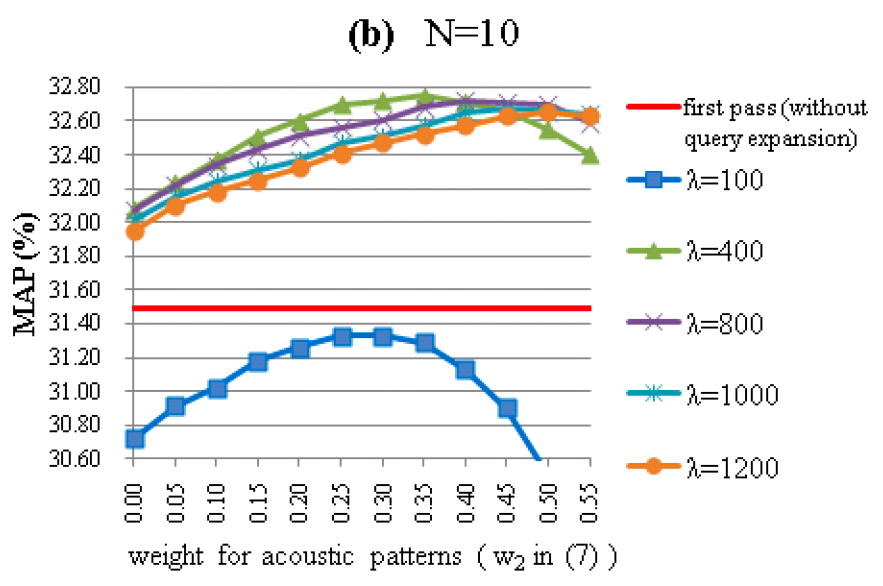
\includegraphics[scale=0.4]{images/chap3_resultb.png}
\caption{將文字形式和聲學組型形式的查詢詞擴展疊加後的平均準確率 ($N=10$)} \label{fig:chap3_resultb}
\end{figure}

圖 ~\ref{fig:chap3_resulta} 和圖 ~\ref{fig:chap3_resultb} 中表示了將文字形式和聲學組型形式的查詢詞擴展疊加後的平均準確率,縱軸為平均準確率(MAP),橫軸為線性疊加中聲學組型的權重。圖中的紅色橫線是第一次檢索結果的平均準確率 (不含查詢詞擴展)。

\section{本章總結}
在本章中使用了聲學組型加強監督式語音文件語意搜索的成效,如此一來可以解決諸如辨識錯誤、語音文件中包含詞典外詞彙的問題,可以有效提升語意檢索的平均準確率。

